\section{Implementation}
%how to validate implementation
\noindent{\bf Persistent memory hardware} We emulate persistent memory using volatile DRAM memory. NVMs are slower than DRAM, so we account for 
slow NVM latency using memory throttling. The modern CPUs allow us to configure the duty cycle value in the memory channel. We use that
facility to throttle the bandwidth of the DRAM memory device, reducing the bandwidth and latency of the DRAM reads/writes. 

\noindent{\bf Persistent containers}
We use persistent data-structure implementations of Intel PMDK to model our persistent containers. The PMDK's goal is not to 
create persistent containers. Hence we had to wrap some of their persistent memory data-structures to fit our container model.
e.g.: Wrapping B+tree with map interface.

\noindent{\bf Data Replication}

We use log replication system software layer called cyclone~\cite{cyclone} for our data replication. Cyclone implements 
state machine replication with Raft as the consensus protocol. Cyclone network transports use highly optimized 
userspace Intel's data plane development kit (DPDK) transport stack. Due to this, we had to port YCSB benchmark to
use same DPDK transport for performance reasons.

\section{Implementation}



\section{Evaluation}
%evaluate performance
We evaluate a prototype version of Blizzard to understand the initial peformance characteristics of the proposed
system. Specifically, we seek to answer the following question -- ``What is the cost of reliable data-structures of
Blizzard comapred to state of the art system storage stacks?. ``

To this end we evaluate the performance of reliable persistent map data structure of Blizzard to a state of the art
key-value store implementation. We describe each of them below.

\noindent{Blizzard persistent-map}
This is a persistent B+tree structure that works with our operations replication layer. The internal nodes
store 64 keys, and maintain sorted ordering at all times. We use copy-on-write (COW) crash consistency 
semantics -- we create a new subtree and copy the data over, whenever we encounter a internal node split. 
We then switch the consistent view of the tree to new subtree using an atomic CAS primtive. 
\noindent{RocksDB}
RocksDB is an open source persistent storage engine by Facebook. It is being used by number of production quality
applications as their persistent storage stack. The key data-structure supporting RocksDB is, log-structured merge
tree (LSM) ~\cite{lsm}. LSM workaround the slow writes of SSD storage device by buffering them on the main memory.
We point both write-ahead-log (WAL) and storage structures (SSTables) of RocksDB to use NVM memory.

\noindent{workload}
We use a YCSB like workload to benchmark these different backends. The client is remote to the replication
cluster and uses DPDK network stack to communicate with the master node. The operations are key-value updates and
reads with configurable ratios between them. The client uses an asynchronous message semantics so that we can
load the target backend server with enough requests.

%testbed
We use a three machine nodes connected with ethernet networking hardware as our testbed. We use real NVM hardware
in our test platform. The workload generator/client sits in a separate node. We list the hardware configuration of
our test bend in ~\autoref{testbed}
\begin{center}
	\begin{tabular}{l|l}
		\hline
		CPU & 1.2 Ghz, 96 cores over 2 NUMA sockets \\
		Network & 100G ethernet LAN \\
		Network-stack & Intel DPDK \\
		DRAM & 256 GB \\
		NVRAM & 1 TB \\
	\end{tabular}
\end{center}

%result analysis

\begin{figure}[tbp]   
	\centering
	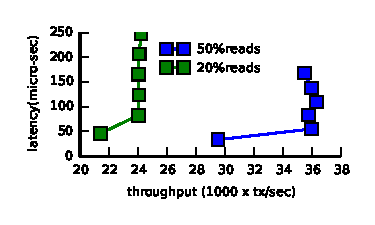
\includegraphics[width=\linewidth]{plot/rocksdbcompare.pdf} 
	\caption{\small RocksDB throughput latency numbers under different read/write ratios. The WAL and the SSTables are placed on NVM} 
	\label{fig:pmemkv} 
\end{figure}

\begin{figure}[tbp]   
	\centering
	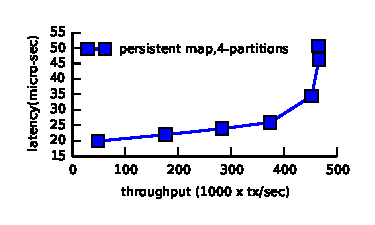
\includegraphics[width=\linewidth]{plot/bliztree-partition.pdf} 
	\caption{\small B-tree based persistent map with 4 partitions/executor threads} 
	\label{fig:pmemkv} 
\end{figure}

%future work
Furthermore,we plan to evaluate our system with a real application workload. In this experiment setup, we try to understand the costs
and benefits involved while using a reliable persistent containers as the basic application's peristent storage abstraction.
We looked in to porting a ``Hackernews`` like web-application to use Blizzard data-structures. The application named Lobsters
~\cite{lobsters} among others, maintain two key tables named ``posts`` and ``votes``. The first table stores the 
title,url,etc related to particular post and the latter stores the individual vote counts for a given post. The original
Lobsters application uses an inner join to between these two tables to derive the output table that has top-most K posts
by votes. We identify that this read pattern can be effectively supported using a more natural in-memory data strucutre --
persistent priority queue. We are working towards that.


\section{Project Goals}
%project goals description
We have identified the following goals for our project.
\begin{itemize}
	\item {\bf The 75$\%$ goal:} 1) Porting a Tree (range lookup) and Map ( point lookup) data structure as a reliable persistent containers. 2) Implementing
			client side library routines to interact with those containers over the network. 

		\item {\bf The 100$\%$ goal:} 1) Port YCSB benchmark to work with our containers. 2) Port a state of the art kv-store (RocksDB). 
				3) Using ported YCSB benchmark client, report numbers for Blizzard containers and competing state of the art. ( RocksDB ).

			\item {\bf The 125$\%$ goal:} Extend and PMWCAS to support reliability. This include design of the primive as it is not straight forward at this
					point to design it.
			\end{itemize}



			\section{Related Work}

			PMWCAS~\cite{pmwcas} is a programming primtive that supports both persistency and multiword updates.
			It extends well known CAS pritmive with multiword support while supporting same all or nothing
			programming semantics of CAS. Furthermore, it extends the CAS to be persistent memory aware by
			adding support for durability semantics ( fences and cache-line flushes).

			Intel PMDK~\cite{pmdk} provides persistent memory aware data-structures. But they lack the reliability semantics.

